\section{实验二：\texttt{SYN} 洪泛攻击与防范}

\subsection{实验环境与网络拓扑}

本实验在实验一已搭建的 VirtualBox 与 OpenWRT 环境上调整网络拓扑，不再需要实验一中的三台隐藏资产。按照实验指导，使用 Attacker 构造 \texttt{TCP SYN} 报文，以 Server 的 \texttt{80/tcp} 端口作为目标，使用 User 检查测试期间 \texttt{HTTP} 服务是否仍可访问。各虚拟机的实际地址及角色见表~\ref{tab:task2-network}，实验拓扑见图~\ref{fig:task2-topology}。

\begin{table}[H]
    \centering
    \caption{\texttt{SYN} 洪泛攻击与防范实验的实际网络配置}
    \label{tab:task2-network}
    \renewcommand{\arraystretch}{1.2}
    \begin{tabularx}{\linewidth}{l l >{\raggedright\arraybackslash}X}
        \toprule
        虚拟机 & 实验使用的 IPv4 地址 & 实验角色及网段 \\
        \midrule
        Attacker & \texttt{192.168.2.100} & 攻击者网段（\texttt{192.168.2.0/24}），构造并发送 SYN 报文 \\
        User & \texttt{192.168.3.100} & 用户网段（\texttt{192.168.3.0/24}），检查 Web 服务响应 \\
        Server & \texttt{192.168.4.105} & 服务器网段（\texttt{192.168.4.0/24}），监听 TCP 80 端口 \\
        OpenWRT & \shortstack[l]{\texttt{192.168.2.1}\\\texttt{192.168.3.1}\\\texttt{192.168.4.1}} & 连接并转发三个网段之间的流量 \\
        \bottomrule
    \end{tabularx}
\end{table}

\begin{figure}[H]
    \centering
    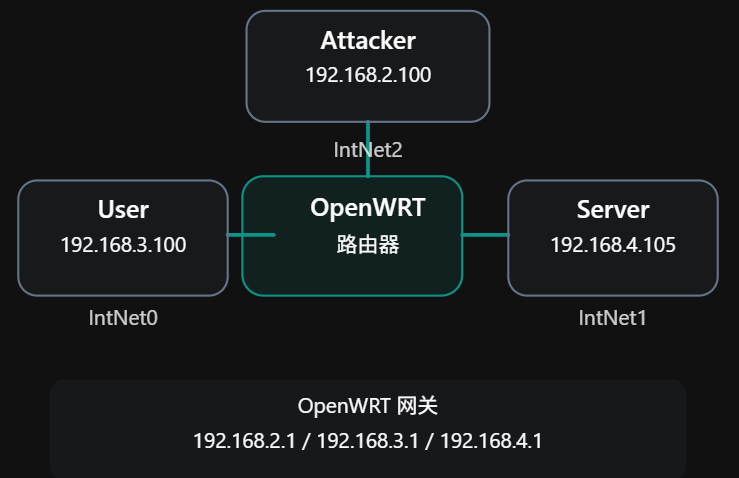
\includegraphics[width=0.87\linewidth]{figures/task12/任务二网络拓扑.png}
    \caption{实验二的网络拓扑：Attacker、User 和 Server 通过 OpenWRT 互联}
    \label{fig:task2-topology}
\end{figure}

与实验一相比，本实验将 User 调整至 \texttt{IntNet0}，地址设为 \texttt{192.168.3.100/24}，经网关 \texttt{192.168.3.1} 访问其他网段；Attacker 保留 \texttt{192.168.2.100}，Server 保留 \texttt{192.168.4.105}。OpenWRT 的 \texttt{eth2}、\texttt{eth3} 和 \texttt{eth1} 分别提供相应网段的网关接口。Server 上的 Apache Web 服务此前已经通过端口扫描确认开放，因此本实验继续使用其 \texttt{80/tcp} 端口进行测试。

\subsection{实验原理与服务器初始状态}

正常的 \texttt{TCP} 三次握手依次交换 \texttt{SYN}、\texttt{SYN+ACK} 和 \texttt{ACK} 报文。当服务器收到客户端的 \texttt{SYN} 报文后，会回复 \texttt{SYN+ACK}，在等待最后一个 \texttt{ACK} 的过程中，相关连接可能表现为 \texttt{SYN\_RECV} 状态。如果大量 \texttt{SYN} 请求无法完成握手，服务器可能产生较多等待中的半连接，占用与未完成连接相关的资源。

\texttt{SYN Cookies} 是针对这种风险的一种防御机制。Linux 在 \texttt{tcp\_syncookies=1} 时，通常在 \texttt{SYN} 队列承受溢出压力后才使用 Cookie 编码连接信息，而不是在每次接收到 \texttt{SYN} 时都立即启用。因此，配置开关的状态与防御机制是否实际触发，是需要区分的两个问题。

在 Server 上先确认 \texttt{80/tcp} 处于监听状态，并检查 \texttt{SYN Cookies} 的初始配置：

\begin{lstlisting}[language=bash,caption={检查服务器监听端口与 SYN Cookies 配置}]
sudo ss -lnt | grep ':80'
sysctl net.ipv4.tcp_syncookies
\end{lstlisting}

实际输出显示服务器在 \texttt{*:80} 上监听，初始 \texttt{net.ipv4.tcp\_syncookies=1}。随后使用 \texttt{ss} 统计半连接数量，作为发包前的观察基线：

\begin{lstlisting}[language=bash,caption={持续观察服务器 TCP 80 端口的半连接数量}]
watch -n 1 "ss -Hant state syn-recv '( sport = :80 )' | wc -l"
\end{lstlisting}

初始观察到的半连接数为 0，结果如图~\ref{fig:task2-before} 所示。实验指导使用 \texttt{netstat -nat | grep SYN\_RECV}，本实验改用功能相近的 \texttt{ss}，并通过 \texttt{wc -l} 统计记录数。

\begin{figure}[H]
    \centering
    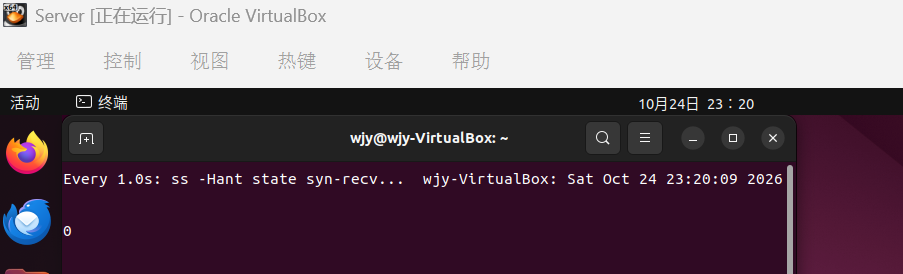
\includegraphics[width=0.87\linewidth]{figures/task12/server上的tcp数目.png}
    \caption{发送测试报文前，Server 的 \texttt{SYN\_RECV} 数量为 0}
    \label{fig:task2-before}
\end{figure}

\subsection{使用 Scapy 构造 \texttt{TCP SYN} 报文}

按照实验指导，在 Attacker 上使用 Scapy 分别构造 IP 层与 TCP 层。目标主机设为 \texttt{192.168.4.105}，目标端口为 80；伪造源 IP 为实验网段中未分配给真实主机的 \texttt{192.168.3.101}，以便在服务器端观察未正常完成握手的连接。随机源端口使不同的测试报文可对应不同的连接四元组。

先创建 \texttt{syn\_test.py}，在第一轮中只发送 30 个报文，检验构造与观察方法是否有效：

\begin{lstlisting}[language=Python,caption={第一轮：构造并发送 30 个 TCP SYN 测试报文}]
from scapy.all import IP, TCP, RandShort, send

source_ip = "192.168.3.101"
target_ip = "192.168.4.105"
target_port = 80

for i in range(30):
    ip_packet = IP(src=source_ip, dst=target_ip)
    tcp_packet = TCP(
        sport=RandShort(),
        dport=target_port,
        flags="S"
    )
    syn_packet = ip_packet / tcp_packet
    send(syn_packet, verbose=False)

print("已完成 30 次 TCP SYN 测试发送")
\end{lstlisting}

其中，\texttt{flags="S"} 只设置 \texttt{SYN} 标志；\texttt{RandShort()} 生成随机 TCP 源端口；\texttt{/} 将 IP 层和 TCP 层封装为完整报文。与实验指导中的 \texttt{loop=1} 持续发送不同，本次先使用有限循环，便于控制测试规模并重复对照。

在 Attacker 上运行：

\begin{lstlisting}[language=bash,caption={在 Attacker 运行 Scapy 脚本}]
sudo python3 syn_test.py
\end{lstlisting}

随后在 Server 上查看具体的半连接记录：

\begin{lstlisting}[language=bash,caption={查看 SYN\_RECV 状态的连接信息}]
sudo ss -ant state syn-recv '( sport = :80 )'
\end{lstlisting}

图~\ref{fig:task2-synrecv} 显示，多条记录的本地地址为 \texttt{192.168.4.105:80}，对端地址为 \texttt{192.168.3.101}，但源端口不同。由此可以确认 Scapy 报文已经到达服务器，且相应连接未完成第三次握手。输出中出现的 \texttt{::ffff:} 是 IPv4 映射地址的显示形式，不改变实际使用的 IPv4 地址。

\begin{figure}[H]
    \centering
    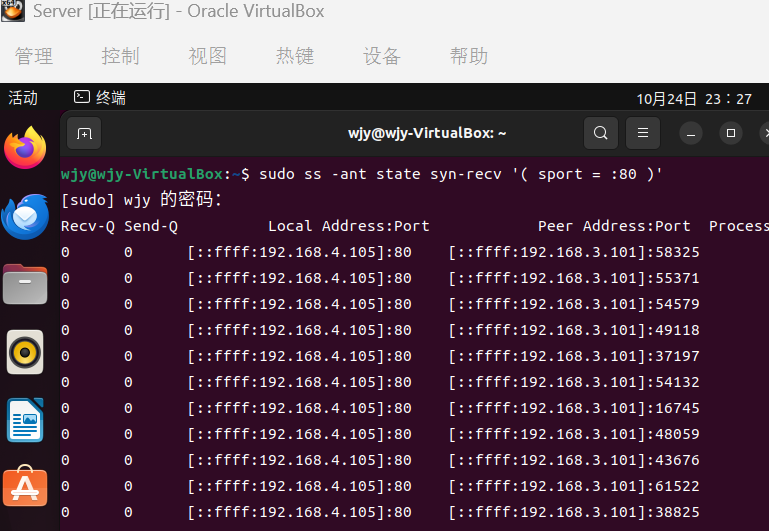
\includegraphics[width=0.88\linewidth]{figures/task12/server上的半连接.png}
    \caption{Server 上观察到来自伪造源地址的 \texttt{SYN\_RECV} 半连接}
    \label{fig:task2-synrecv}
\end{figure}

\subsection{第一轮试探：30 个 SYN 未观察到防御差异}

为按照实验指导比较 \texttt{SYN Cookies} 的作用，先在 Server 上临时关闭该机制，确认配置为 0：

\begin{lstlisting}[language=bash,caption={暂时关闭 SYN Cookies}]
sudo sysctl -w net.ipv4.tcp_syncookies=0
sysctl net.ipv4.tcp_syncookies
\end{lstlisting}

关闭操作与发包前的监测情况见图~\ref{fig:task2-off}。在对照测试中还将 \texttt{watch} 刷新间隔缩短为 0.2 秒，尽量减少遗漏短时变化的可能。待先前的半连接消退后，在 Attacker 再次运行同一个 \texttt{syn\_test.py}，Server 实测最多观察到 30 条半连接，如图~\ref{fig:task2-off-30} 所示。

\begin{figure}[H]
    \centering
    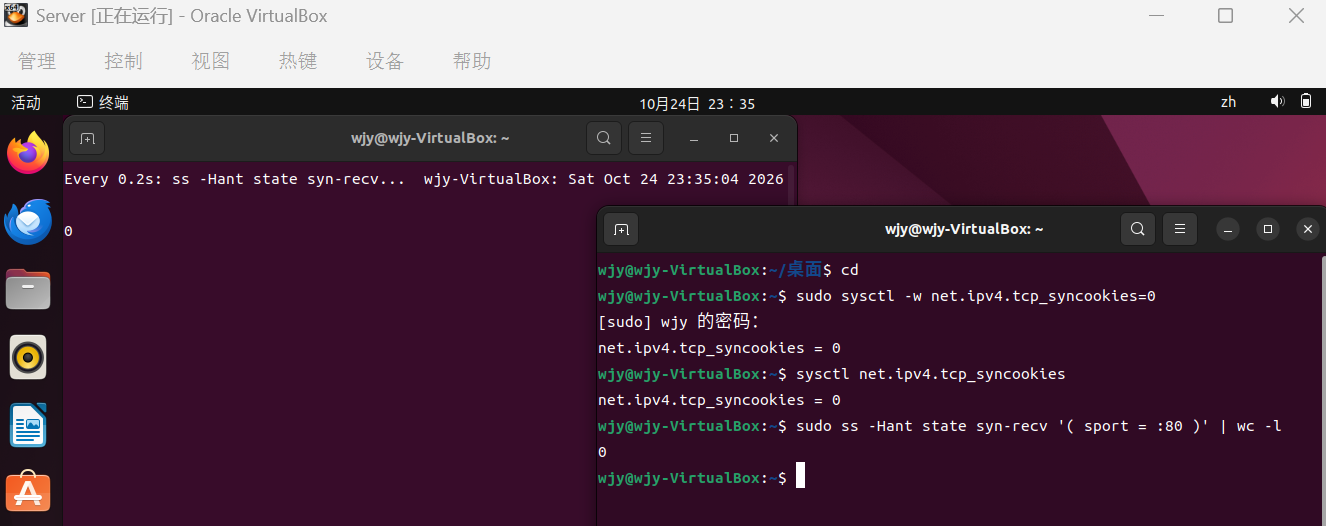
\includegraphics[width=0.86\linewidth]{figures/task12/关闭cookies.png}
    \caption{Server 将 \texttt{SYN Cookies} 设为 0，并准备观察半连接数量}
    \label{fig:task2-off}
\end{figure}

\begin{figure}[H]
    \centering
    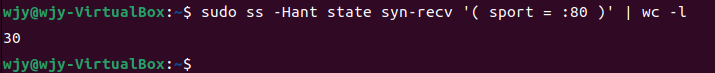
\includegraphics[width=0.76\linewidth]{figures/task12/运行30次攻击脚本后，观察server.png}
    \caption{关闭 \texttt{SYN Cookies} 后，30 次 \texttt{SYN} 测试出现 30 条半连接}
    \label{fig:task2-off-30}
\end{figure}

接着开启 \texttt{SYN Cookies}，配置值设为 1，仍使用相同的 30 次发包脚本：

\begin{lstlisting}[language=bash,caption={开启 SYN Cookies 并检查发送计数器}]
sudo sysctl -w net.ipv4.tcp_syncookies=1
sysctl net.ipv4.tcp_syncookies
nstat -az | grep TcpExtSyncookies
\end{lstlisting}

如图~\ref{fig:task2-on} 与图~\ref{fig:task2-on-30} 所示，开启后再次发送 30 个 \texttt{SYN} 报文，Server 仍观察到 30 条半连接，\texttt{TcpExtSyncookiesSent} 计数器没有增加。

\begin{figure}[H]
    \centering
    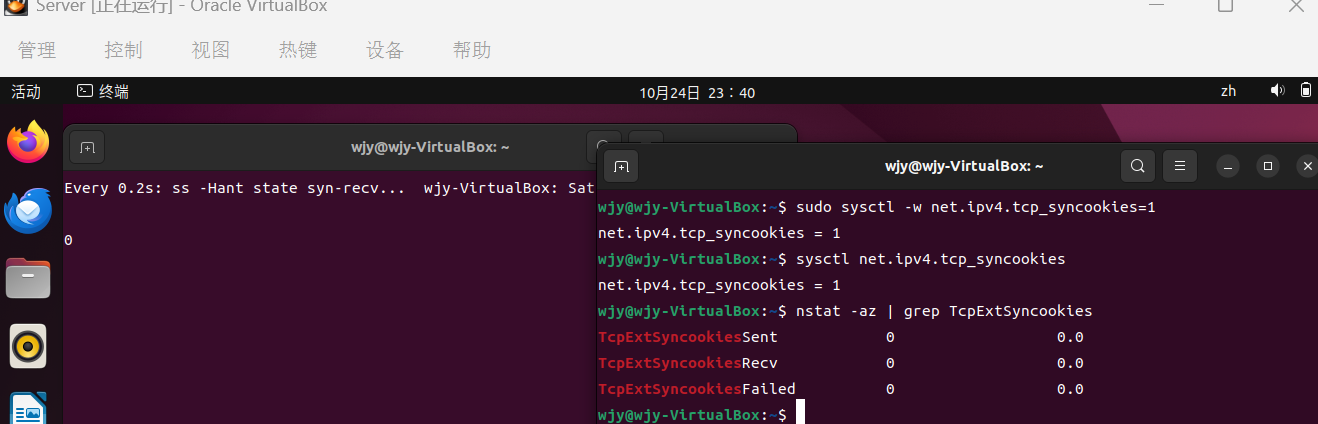
\includegraphics[width=0.86\linewidth]{figures/task12/开启cookies.png}
    \caption{Server 开启 \texttt{SYN Cookies} 并检查相关计数器}
    \label{fig:task2-on}
\end{figure}

\begin{figure}[H]
    \centering
    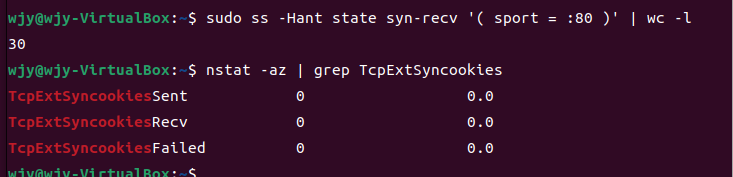
\includegraphics[width=0.83\linewidth]{figures/task12/再次运行30遍攻击脚本.png}
    \caption{开启 \texttt{SYN Cookies} 后，30 次测试仍为 30 条半连接，发送计数未增加}
    \label{fig:task2-on-30}
\end{figure}

同时，从 User 使用 \texttt{curl} 检查服务器的 HTTP 响应：

\begin{lstlisting}[language=bash,caption={由 User 测试服务器 HTTP 服务是否可用}]
curl -I --max-time 5 http://192.168.4.105
\end{lstlisting}

实际收到 \texttt{HTTP/1.1 401 Unauthorized}，如图~\ref{fig:task2-http} 所示。由于服务器原本就采用 HTTP Digest 身份认证，此状态码说明服务器已正常响应 HTTP 请求，并不是服务中断。

\begin{figure}[H]
    \centering
    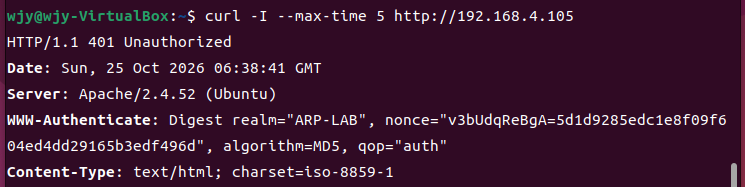
\includegraphics[width=0.84\linewidth]{figures/task12/测试web.png}
    \caption{30 次 \texttt{SYN} 测试后，Server 仍能返回 HTTP 401 响应}
    \label{fig:task2-http}
\end{figure}

\textbf{第一轮遇到的问题在于：}虽然成功构造了报文并观察到半连接，但关闭和开启 \texttt{SYN Cookies} 后，\texttt{SYN\_RECV} 数量均为 30，且 Cookie 发送计数没有增加，两组结果无法体现明显的防御差异。结合 \texttt{tcp\_syncookies=1} 的工作条件，推测 30 个报文尚未使服务器半连接队列承受足够压力。因此，这一轮完成了半连接机制验证，\emph{但没有达到观察 SYN Cookies 防御差异的预期}。

\subsection{第二轮调整：增加至 500 个 SYN 进行对照}

为了继续完成实验指导中“比较开启与关闭 SYN Cookies 时服务器半连接数量”的要求，本实验先查看系统的相关队列参数，实际得到 \texttt{tcp\_max\_syn\_backlog=256}、\texttt{somaxconn=4096}。这些参数说明内核存在相应的队列容量设置，但不能将其中任一数值直接视为 \texttt{SYN\_RECV} 统计的固定上限。随后保持目的地址、目标端口和报文结构不变，仅将脚本中的发送循环次数从 30 增加到 500，以尝试扩大服务器的半连接压力。调整后的关键代码如下：

\begin{lstlisting}[language=Python,caption={第二轮仅修改测试循环次数}]
for i in range(500):
    ip_packet = IP(src=source_ip, dst=target_ip)
    tcp_packet = TCP(
        sport=RandShort(),
        dport=target_port,
        flags="S"
    )
    send(ip_packet / tcp_packet, verbose=False)

print("已完成 500 次 TCP SYN 测试发送")
\end{lstlisting}

\subsubsection{关闭 SYN Cookies 时的测试}

首先在 Server 上设置 \texttt{net.ipv4.tcp\_syncookies=0}，在此前半连接基本消退后，Attacker 运行修改后的脚本。Attacker 的执行结果见图~\ref{fig:task2-send-500}，Server 观察到的最大 \texttt{SYN\_RECV} 数量为 193，如图~\ref{fig:task2-off-500} 所示。

\begin{figure}[H]
    \centering
    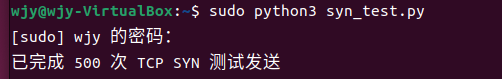
\includegraphics[width=0.76\linewidth]{figures/task12/运行500次攻击脚本.png}
    \caption{Attacker 完成 500 次 \texttt{TCP SYN} 测试发送}
    \label{fig:task2-send-500}
\end{figure}

\begin{figure}[H]
    \centering
    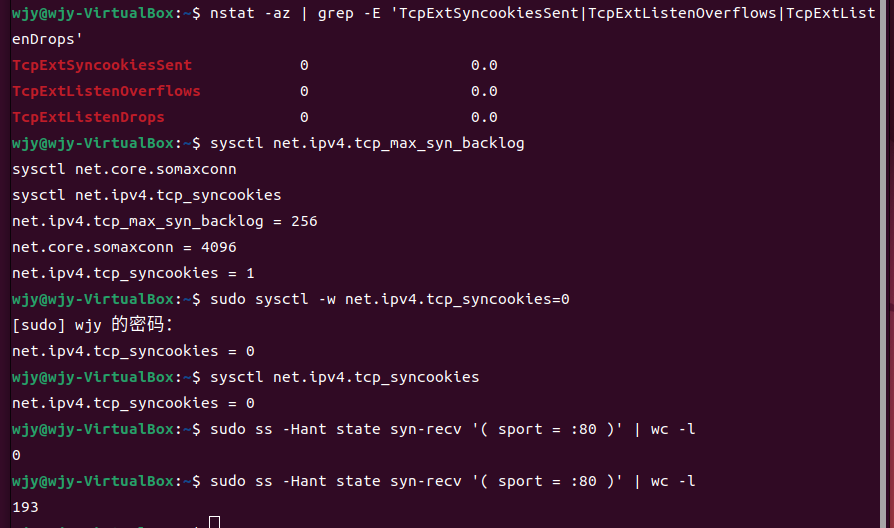
\includegraphics[width=0.88\linewidth]{figures/task12/关闭时，193条半连接.png}
    \caption{关闭 \texttt{SYN Cookies} 时，观测到的最大半连接数为 193}
    \label{fig:task2-off-500}
\end{figure}

这一结果没有达到发送数量 500，说明“发送了 500 个 SYN”与“同时存在 500 条半连接”并不等价；已建立的半连接状态会随报文到达时间、服务器处理过程及超时而变化。User 此时再次访问 Web 服务，仍收到 HTTP 401 响应，结果见图~\ref{fig:task2-http-500}。

\begin{figure}[H]
    \centering
    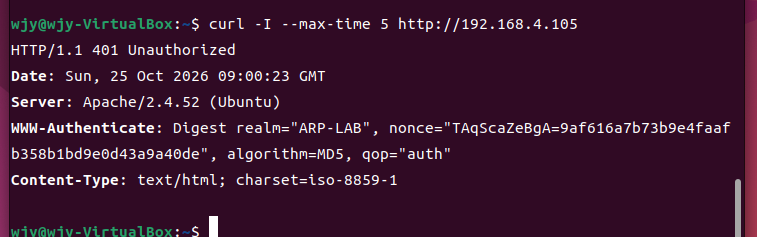
\includegraphics[width=0.84\linewidth]{figures/task12/web响应仍然正常.png}
    \caption{500 次测试且关闭 \texttt{SYN Cookies} 时，HTTP 服务仍正常响应}
    \label{fig:task2-http-500}
\end{figure}

\subsubsection{开启 SYN Cookies 时的测试}

之后在 Server 上将 \texttt{net.ipv4.tcp\_syncookies} 恢复为 1，如图~\ref{fig:task2-on-again} 所示。待上一轮半连接消退后，再次运行相同的 500 次发送脚本。本次观察到的最大 \texttt{SYN\_RECV} 数量为 385，对应结果见图~\ref{fig:task2-on-500}。根据实验记录，此时 User 的 HTTP 服务访问仍正常。

\begin{figure}[H]
    \centering
    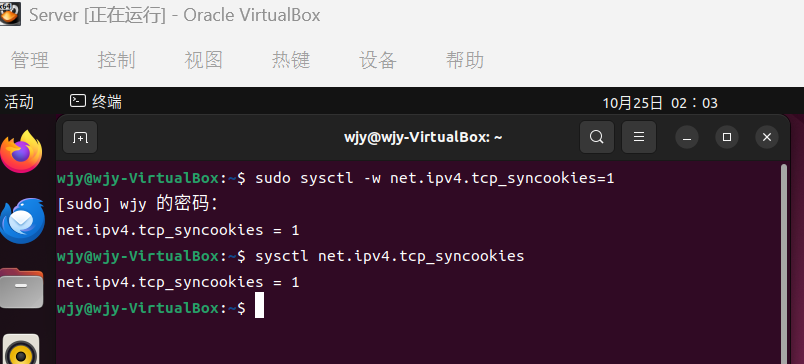
\includegraphics[width=0.82\linewidth]{figures/task12/再次开启cookies.png}
    \caption{第二轮对照中重新开启 \texttt{SYN Cookies}，配置值为 1}
    \label{fig:task2-on-again}
\end{figure}

\begin{figure}[H]
    \centering
    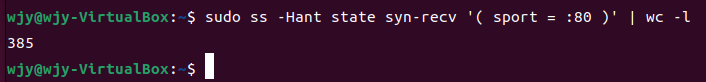
\includegraphics[width=0.79\linewidth]{figures/task12/再次运行500次.png}
    \caption{开启 \texttt{SYN Cookies} 时，500 次测试观测到 385 条半连接}
    \label{fig:task2-on-500}
\end{figure}

两轮测试的结果整理如表~\ref{tab:task2-results} 所示。

\begin{table}[H]
    \centering
    \caption{不同发送规模与 SYN Cookies 配置下的实验结果}
    \label{tab:task2-results}
    \renewcommand{\arraystretch}{1.2}
    \begin{tabularx}{\linewidth}{c c c c X}
        \toprule
        发送规模 & SYN Cookies & 最大观察 \texttt{SYN\_RECV} & HTTP 响应 & Cookie 发送计数 \\
        \midrule
        30 & 关闭（0） & 30 & 正常 & 未作为该组指标记录 \\
        30 & 开启（1） & 30 & 正常 & \texttt{SyncookiesSent} 未增加 \\
        500 & 关闭（0） & 193 & 正常 & 未作为该组指标记录 \\
        500 & 开启（1） & 385 & 正常 & 未记录测试前后增量 \\
        \bottomrule
    \end{tabularx}
\end{table}

\subsection{实验现象及问题分析}

\subsubsection{为什么 30 次试探未成功体现防御差异？}

第一轮发送 30 个 \texttt{SYN} 时，服务器已经产生了 30 条半连接，说明 Scapy 脚本构造和网络转发正常，\texttt{TCP} 握手未完成的状态也得到验证。这里所谓“失败”，并非脚本发送失败或无法制造半连接，而是\textbf{未能观察到 SYN Cookies 开启前后的明显差异}。

当 \texttt{tcp\_syncookies=1} 时，Linux 通常在未完成连接队列出现溢出压力后才使用 SYN Cookie。由于 30 次测试的压力较低，开启配置后服务器仍然可以按通常方式维护半连接，因此两组 \texttt{SYN\_RECV} 数量相同，且在该轮观察到的 \texttt{SyncookiesSent} 没有增加。这也是后续提高测试数量的直接原因。


\subsubsection{思考题：为什么开启 SYN Cookies 前后 SYN\_RECV 数量存在差异？（这里以500轮试探为例）}

SYN Cookies 是一种针对 SYN Flood 攻击的防御机制。在正常的 TCP 三次握手过程中，服务器收到客户端发送的 SYN 报文后，会回复 SYN-ACK 报文，并为尚未完成握手的连接维护相应状态，使其进入 \texttt{SYN\_RECV}。当大量 SYN 报文持续到达而最终 ACK 未能返回时，半连接不断积累，可能造成 SYN 队列溢出，进而影响正常客户端建立连接。

当 SYN Cookies 关闭时，服务器主要依靠常规半连接队列维护这些连接状态；当 SYN Cookies 开启时，Linux 通常在 SYN 队列发生溢出时启用该机制，将必要的连接信息编码到 SYN-ACK 报文的初始序列号中，从而减少对常规半连接状态的依赖。因此，\textbf{SYN Cookies 的核心作用是在队列承受压力时降低半连接状态维护的开销，而非直接清空已有的半连接。} 即使开启该机制，服务器仍可能存在一定数量的 \texttt{SYN\_RECV} 连接。

在本次实验的第一轮测试中，分别在开启和关闭 SYN Cookies 的条件下发送 30 个 SYN 报文，观察到的最大半连接数量均为 30，且未观察到 SYN Cookie 发送计数增加。这表明较低的测试负载尚未使服务器产生明显的队列压力，因此两组结果没有表现出明显差异。

为进一步观察不同配置下的实验现象，第二轮将 SYN 报文数量增加至 500。实验结果显示，关闭 SYN Cookies 时最大观察到 193 条半连接，开启时最大观察到 385 条半连接。与第一轮相比，两组结果出现了更加明显的数量差异，且变化方向与实验指导中的示例现象相似。因此，从\textbf{实验观察与对照}的角度来看，增加测试规模后得到了更有辨识度的结果。

但是，\texttt{SYN\_RECV} 数量不仅受到 SYN Cookies 配置的影响，还与 SYN 报文的实际到达速率、TCP 重传与超时机制、不同测试轮次的队列状态以及 \texttt{watch} 命令的周期性采样时刻等因素有关。此外，SYN Cookies 开启后并不会自动删除已有半连接，因此不能简单认为开启该功能后 \texttt{SYN\_RECV} 数量一定减少，也不能仅凭本次实验中 ``385 大于 193'' 的现象认定 SYN Cookies 已经触发，或者认为开启该功能会导致半连接数量增加。

进一步而言，由于第二轮实验未记录 \texttt{TcpExtSyncookiesSent} 计数器在测试前后的变化，因此尚缺少直接证明 SYN Cookies 实际触发的证据。同时，两组测试中服务器的 HTTP 服务均能够正常响应，说明当前测试条件下尚未观察到明显的拒绝服务现象。

综上所述，\textbf{SYN Cookies 开启前后 \texttt{SYN\_RECV} 数量的差异，是半连接队列管理机制、报文到达情况及连接超时等多种因素共同作用的结果。} 本次实验成功观察到随着 SYN 请求数量增加，服务器半连接状态发生了明显变化，但不能仅根据半连接数量判断 SYN Cookies 的实际防御效果，还需要结合 SYN Cookie 发送计数器及正常服务的可用性进行综合分析。
